\documentclass[12pt]{article}
\usepackage{geometry}
\geometry{a4paper, margin=1in}
\usepackage{graphicx}
\usepackage{hyperref}
\usepackage{fancyhdr}
\usepackage{listings}
\usepackage{amsmath}

\pagestyle{fancy}
\fancyhf{}
\rhead{Arbitrary Precision Arithmetic Library}
\lhead{Project Report}
\rfoot{Page \thepage}

\title{Arbitrary Precision Arithmetic Library}
\author{Amogh Bindal\\ ES23BTECH11004}
\date{\today}

\begin{document}

\maketitle

\section{Introduction}

While developing these files, my primary goal was to implement arbitrary-precision arithmetic for both integers and floating-point numbers in Java. I started with the AInteger class to handle large integers, including negative values, and then extended this functionality to floating-point numbers with the AFloat class.

For AInteger, I focused on representing numbers as strings to bypass the limitations of Java’s built-in numeric types. I implemented methods for basic arithmetic operations-addition, subtraction, multiplication, and division-by simulating manual algorithms (similar to how calculations are done by hand). Special care was taken to manage leading zeros, negative numbers, and edge cases like division by zero. The class also includes utility methods for parsing and normalizing input.

Building on AInteger, I created the AFloat class to support arbitrary-precision floating-point arithmetic. This class inherits from AInteger and adds fields to track the number of digits after the decimal point and the value without the decimal. Arithmetic operations in AFloat align the decimal points before performing calculations using the underlying integer logic from AInteger. The results are then formatted correctly with the decimal point. This design allows for precise calculations with very large or very small floating-point numbers, handling sign and scale adjustments as needed.

\section{Design Overview}
This project consists of two core classes: \texttt{AInteger} and \texttt{AFloat}, built to perform arbitrary-precision integer and floating-point arithmetic respectively. Key design features include:
\begin{itemize}
    \item Support for large numbers without precision loss.
    \item Manual implementation of basic arithmetic: addition, subtraction, multiplication, and division.
    \item Separation of integer and decimal components in \texttt{AFloat} to aid high-precision operations.
    \item Used Basic Multiplicatoin and long Division algorithms to carry out the calculations
\end{itemize}

\subsection*{UML Diagram}
\begin{center}
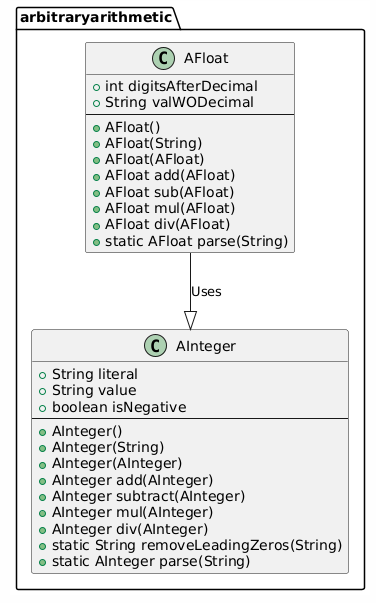
\includegraphics[width=0.5\textwidth]{uml-diagram.png}
\end{center}

\section{How to Use the Library}
\subsection{How to run in a java file}
\begin{verbatim}
1. Import the classes in your Java project:
   import arbitraryarithmetic.AInteger;
   import arbitraryarithmetic.AFloat;

2. Create objects:
   AInteger a = new AInteger("12345678901234567890");
   AFloat b = new AFloat("3.1415926535");

3. Use methods:
   AInteger result = a.add(new AInteger("100"));
   AFloat fresult = b.mulF(new AFloat("2.5"));

4. Run the main methods in each class for examples.

\end{verbatim}
\subsection{Running using Docker}

To run the project using Docker, we first create a Docker image that uses Java 21 and Apache Ant. The Dockerfile compiles the Java code using Ant and sets the built JAR file as the container entry point.

\begin{itemize}
    \item \textbf{Build the image:}
    \begin{verbatim}
    docker build -t myinfarith .
    \end{verbatim}

    \item \textbf{Pull from DockerHub}
    \begin{verbatim}
        docker image pull amoghbindal/myinfarith
    \end{verbatim}

    \item \textbf{Run the container:}
    \begin{verbatim}
    docker run -it amoghbindal/myinfarith int add 123 456
    \end{verbatim}
\end{itemize}

This command runs the image and gives us access to the interactive shell in the image.

\subsection{Running using Python and CLI}

A Python script named \texttt{run\_myinfarith.py} is provided to compile the project using Ant and execute the generated JAR file with command-line arguments.

\begin{itemize}
    \item \textbf{Run the program:}
    \begin{verbatim}
    python run_myinfarith.py float mul 3.14 2.0
    \end{verbatim}
\end{itemize}

This internally runs:
\begin{itemize}
    \item \texttt{ant jar} to build the project.
    \item \texttt{java -jar dist/MyInfArith.jar} with provided arguments.
\end{itemize}

\subsection{Running using Ant}

The project can also be built and executed directly using Apache Ant. A \texttt{build.xml} file is included which automates the compilation and packaging.

\begin{itemize}
    \item \textbf{Build the JAR file:}
    \begin{verbatim}
    ant jar
    \end{verbatim}

    \item \textbf{Run the program:}
    \begin{verbatim}
    java -jar dist/MyInfArith.jar int sub 100 45
    \end{verbatim}
\end{itemize}

The build process compiles all Java source files into the \texttt{build/} directory and creates a JAR file in the \texttt{dist/} directory.


\section{Git Commit Snapshot}
\begin{itemize}
    \item Please refer to the included image \texttt{gitlog.png} for a snapshot of commit history.
\end{itemize}
\begin{center}
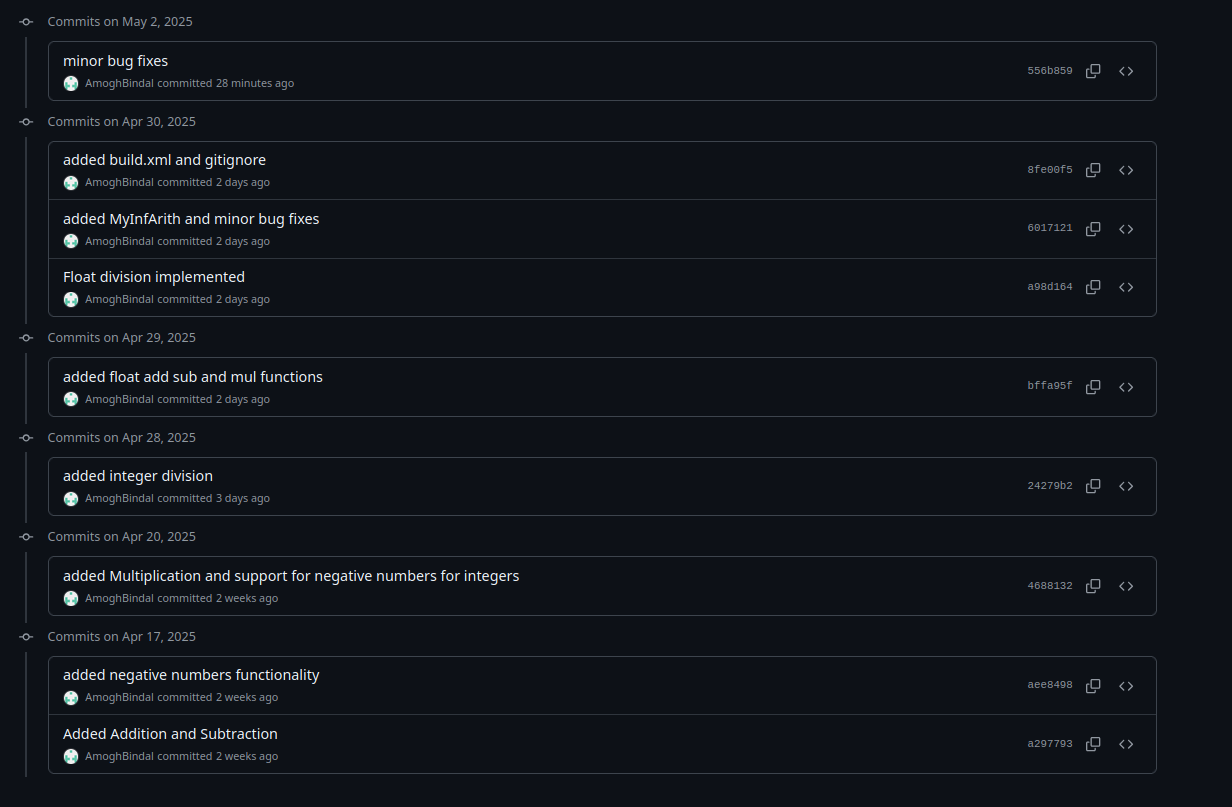
\includegraphics[width=0.9\textwidth]{gitlog.png}
\end{center}

\section{Limitations}
\begin{itemize}
    \item Performance may degrade with extremely large inputs due to use of string-based arithmetic.
    \item Floating point division is manually padded for precision but not dynamically adaptive.
    \item There are better/faster methods to implement for division and multiplication
    \item No input validation for malformed strings beyond basic error checks.
    \item Leading zeros of decimal values not removed
    \item Can't change precision of the decimal easily and it is 30 rightnow which may not be enough sometimes9
    \item The function a.add(b) will not not update the value of a. (It is very easy to solve by using a set method to set the value of 2 objects to be equal we can set the attributes of the result after each operation equal to the instances attributes.)
\end{itemize}

\section{Verification Approach}
\begin{itemize}
    \item Manual test cases written in \texttt{main()} methods for both classes.
    \item Verifications include negative inputs, large numbers, and zero-edge cases.
    \item The outputs of operations were cross-verified with Java’s built-in \texttt{BigInteger} and \texttt{BigDecimal}.
\end{itemize}

\section{Key Learnings}

This project provided valuable insights into both software development and tooling practices. The key takeaways include:

\begin{itemize}

    \item \textbf{Java Build Automation with Ant:} Using Apache Ant to compile and package the project helped in understanding XML-based build configuration, and how to automate repetitive compilation and packaging tasks.

    \item \textbf{Containerization with Docker:} Creating a Dockerfile to encapsulate the Java runtime, Ant environment, and project code emphasized the importance of reproducibility and portability in software deployment.

    \item \textbf{CLI Application Design:} Designing a command-line interface for invoking arithmetic operations improved understanding of argument parsing and user input validation in Java.

    \item \textbf{Cross-language Integration:} Writing a Python script to build and run the Java project demonstrated how scripting languages can be used to automate and streamline workflows.

    \item \textbf{Version Control Best Practices:} Using Git to track changes across multiple files and features improved code organization and encouraged modular, incremental development.

\end{itemize}


\end{document}
